%\documentclass[AER, draftmode]{AEA}
 \documentclass[oneside,11pt]{article}

% \usepackage{soul}
% \usepackage{natbib}
% \usepackage{hyperref}
% \usepackage{graphicx}             
% \graphicspath{{./paper/Figuras/}}

% \usepackage{float}                
% \usepackage{amsmath}
% \usepackage{amscd}
% \usepackage{amsfonts}
% \usepackage{amssymb}
% \usepackage{bbm}
% \usepackage{booktabs}
% \usepackage{nameref}
% \usepackage{multirow}
% \usepackage[nokeyprefix]{refstyle}
% \usepackage{rotating}
% \usepackage{threeparttable}
% \usepackage{lscape}
% \usepackage{enumerate}
% \usepackage{afterpage}
% \usepackage{caption}
% \usepackage{subcaption}
% \usepackage{epstopdf}
% \epstopdfDeclareGraphicsRule{.tiff}{png}{.png}{convert #1 \OutputFile}
% \AppendGraphicsExtensions{.tiff}

% \epstopdfDeclareGraphicsRule{.tif}{png}{.png}{convert #1 \OutputFile}
% \AppendGraphicsExtensions{.tif}

% \usepackage{tikz}
% \usetikzlibrary{shapes.geometric, arrows}
% \usetikzlibrary{calc}

% \usepackage{colortbl}

% \newtheorem{theorem}{Theorem}
% \newtheorem{claim}[theorem]{Claim}

\onehalfspacing

%%% HELPER CODE FOR DEALING WITH EXTERNAL REFERENCES
\usepackage{xr}
\makeatletter
\newcommand*{\addFileDependency}[1]{
  \typeout{(#1)}
  \@addtofilelist{#1}
  \IfFileExists{#1}{}{\typeout{No file #1.}}
}
\makeatother


\newcommand*{\myexternaldocument}[1]{
    \externaldocument{#1}
    \addFileDependency{#1.tex}
    \addFileDependency{#1.aux}
}

%\myexternaldocument{OA}
%----------------------------------------------------------------

\begin{document}

\begin{titlepage}
\title{Lawyer Quality}
\author{Joyce Sadka\thanks{Instituto Tecnológico Autónomo de México} \and Enrique Seira\thanks{Instituto Tecnológico Autónomo de México} \and Christopher Woodruff\thanks{University of Oxford}}
\date{\today}
\maketitle
\begin{abstract}
\noindent 

\bigskip
\end{abstract}
\setcounter{page}{0}
\thispagestyle{empty}
\end{titlepage}
\pagebreak \newpage

\subsection{Context} 
The poor in developing countries have little access to justice. Courts are ineffective and corrupt, and the market for legal services is inefficient and plagued by poor quality representation. Mexican labor courts are emblematic of these issues. Using firing and lawsuit data, we estimate that fewer than 5\% of Mexico’s dismissed workers even attempt to seek justice through the courts. Among those who do, most recover a small share of what they are owed and more than one-third recover nothing at all. \\

-Insufficient information: Workers are misinformed and excessively optimistic. Only one-third of workers understand their legal entitlements; workers on average believe their probability of winning is 89\%, though only 24\% receive compensation after a judge’s decision. Many workers use low quality, informal lawyers found at the courthouse entrance –commonly called “Coyotes” – instead of acquiring quality legal representation (Sadka et al. 2019). \\

-Lawyers exploit asymmetric information: Lawyers are well compensated for filing a suit, so low-quality lawyers convince workers to sue even if they are unlikely to win and would be better off settling (Sadka et al. 2020). On average, workers recover half of the legal entitlement, and only 20\% of their claim. \\

There is no database workers can consult for lawyers and their outcomes, so plaintiff’s lawyers have weak incentives to acquire reputation. And finally, ignorance and overconfidence may make workers easy prey to lawyers. 

\section{Measuring quality}


We face the significant challenge of measuring the quality of the lawyers. We document quality using distinct information about the casefile. One option is to wait until the cases are all completed and measure the effects on outcomes - we will call this \textbf{objective measures of quality}. There are at least two concerns with measuring quality in this manner. First, higher quality lawyers may handle more difficult cases (Dranove et al, 2003). Second, cases proceeding to judgment may take four years or longer to be completed (Sadka et al., 2019); hence we would need to wait a very long time to measure outcomes.  


The other option, which we refer to as \textbf{subjective measure of quality}, is to assess the quality of the initial case filings\footnote{Measuring the quality in initial case files is a good first approach to measure both case file and lawyer quality because it is a crucial document that determines the principal action in the case, as well as the alleged facts. It is also fairly short, and available at the very beginning of the lawsuit, which allows us to rate both historical casefiles and ongoing casefiles with the same methodology.}, which we view as being determined by the quality of the lawyer and the ability of the plaintiff to monitor the lawyer. Our measure of the quality of the initial case filing is grounded in an incentivized, blind rating of case files by eight lawyers with experience litigating in labor court.


\section{Data}

We have several sources of data. Given the duration of the average lawsuit, in order to create the objective measure of quality we focus on cases filed in 2011, the earliest year for which the court had digital records of all initial case filings. We have data on ~5000 cases. Our second source of data are a subsample of cases filed in all 20 subcourts from May 15, 2017 through 2019\footnote{xxx\% of this cases are still ongoing.} This are the lawsuits rated by experts, and from which we construct the subjective measure of quality.


\section{Objective measures of quality}

Figure \ref{heterogeneity} documents heterogeneity in objective measures of quality. For the different outcomes, we estimate the following specification

\[ \widetilde{y}_i = \alpha X + \sum_j\beta_j\mathds{1}(\text{Lawyer} = j) + \epsilon_j\]

where $\widetilde{y}_i$ is the $z$-score of an objective outcome for casefile $i$, $X$ are casefile controls, and $\beta_j$ is the fixed-effect of lawyer $j$, and we cluster at the lawyer level. The different point estimates $\beta_j$ can be mapped to a score, and we standardize it in such a way that a higher score means a higher quality lawyer. 


\begin{figure}[H] 
    \label{heterogeneity}
    \caption{Lawyer quality heterogeneity (objective)}
     \begin{center}
    \begin{subfigure}{0.49\textwidth}
        \caption{Amount won}
        \centering
        \includegraphics[width=\textwidth]{Figuras/betas_ql_liq_total.pdf}
    \end{subfigure}
    \begin{subfigure}{0.49\textwidth}
        \caption{Recovered a positive amount}
        \centering
        \includegraphics[width=\textwidth]{Figuras/betas_ql_pos_rec.pdf}
    \end{subfigure}
    \begin{subfigure}{0.49\textwidth}
        \caption{Duration}
        \centering
        \includegraphics[width=\textwidth]{Figuras/betas_ql_pos_rec.pdf}
    \end{subfigure}    
 \begin{subfigure}{0.49\textwidth}
        \caption{Amount won as percentage of legal entitlement}
        \centering
        \includegraphics[width=\textwidth]{Figuras/betas_ql_win_minley.pdf}
    \end{subfigure}    
 \begin{subfigure}{0.49\textwidth}
        \caption{Settlement}
        \centering
        \includegraphics[width=\textwidth]{Figuras/betas_ql_settlement.pdf}
    \end{subfigure}        
    \end{center}
    \scriptsize{ \noindent 
    \textit{Do file: }  \texttt{fe\_quality\_betas.do}}

\end{figure}

When dealing with several measures of a latent variable, it is sometimes useful to reduce dimensionality with principal component analysis (PCA), which we do. The following figure is a histogram for the first principal component of the 5 objective measures above.




\begin{figure}[H] 
    \label{pca_hist}
    \caption{Histogram of PCA}
     \begin{center}
      \begin{subfigure}{0.75\textwidth}
        \centering
        \includegraphics[width=\textwidth]{Figuras/hist_pca.pdf}
    \end{subfigure}
    \end{center}
    \scriptsize{ \noindent 
    \textit{Do file: }  \texttt{fe\_quality\_betas.do}}

\end{figure}


The next table shows the correlation between the distinct measures of objective quality.


\begin{table}[H]
    \caption{Correlation objective measures}
    \label{betas_cor}
     \begin{center}
    \scriptsize{% Table generated by Excel2LaTeX from sheet 'betas_cor'
\begin{tabular}{l|cccccc}
\toprule
\multicolumn{1}{r}{} & \multicolumn{1}{l}{PCA} & \multicolumn{1}{l}{Amount won} & \multicolumn{1}{l}{Pos recovery} & \multicolumn{1}{l}{Duration} & \multicolumn{1}{l}{Amount won/Entitlement } & \multicolumn{1}{l}{Settlement} \\
\midrule
\midrule
PCA   & 1     &       &       &       &       &  \\
Amount won & 0.58* & 1     &       &       &       &  \\
Pos recovery & 0.92* & 0.33* & 1     &       &       &  \\
Duration & 0.36* & -0.03 & 0.31* & 1     &       &  \\
Amount won/Entitlement  & 0.81* & 0.6*  & 0.58* & 0.21* & 1     &  \\
Settlement & 0.9*  & 0.29* & 0.97* & 0.32* & 0.53* & 1 \\
\bottomrule
\bottomrule
\end{tabular}%
}
    \end{center}
  \scriptsize{ \noindent 
    \textit{Do file: }  \texttt{fe\_quality\_betas.do}}
\end{table}




\section{Subjective measures of quality}

 




% Instead, we pursue an alternative approach, based on rating the quality of the initial case filing itself. Discussions with lawyers indicated that case filing varied in quality, with issues related to specificity of the information and claims being the most important. For example, is the address of and other contact information for the defendant complete and detailed? Defendants must be served notice of the suit and hearings, and incomplete information is the most common obstacle to timely notification. Are the circumstances of the dismissal complete, including the names and positions of the individuals who carried out the dismissal? These facts about the dismissal are often the main focus of the evidentiary phase of the lawsuit; greater specificity and clarity are key to lawsuit quality. 

% 




% With these issues in mind, we measure the quality of the case filing in four steps. First, we selected a sample of 500 of the 5000 cases filed in 2011 and hired eight licensed lawyers to rate the quality of the initial filing for those cases. Second, we hired two lawyers as consultants. We asked those two lawyers to examine 100 case files and to suggest hard measures that we could objectively code that might be used to judge the quality of the case filing. Third, we code a subset of those 100 objective measures for all of the 500 case files rated by the eight lawyers.


% The lawyers rated each of five main parts of the case filing: the introduction; the list of claims; the facts; the legal arguments; and the closing petitions to the court. They also provided a global rating of the quality of the case filing. They were instructed to rate the case filing itself rather than the quality of the underlying case. The instructions clearly mentioned coherence, completeness, specificity, and well posed claims and arguments as the correct basis for the evaluation, rather than the value of the case or the legal merits of the case


\begin{figure}[H] 
    \label{}
    \caption{Distribution of ratings}
     \begin{center}
      \begin{subfigure}{0.49\textwidth}
        \caption{Total Score}
        \centering
        \includegraphics[width=\textwidth]{Figuras/hist_total.pdf}
    \end{subfigure}
    \begin{subfigure}{0.49\textwidth}
        \caption{Chapter of Rubro \& Proemio}
        \centering
        \includegraphics[width=\textwidth]{Figuras/hist_calif_rubro_proemio.pdf}
    \end{subfigure}
    \begin{subfigure}{0.49\textwidth}
        \caption{Chapter of benefits}
        \centering
        \includegraphics[width=\textwidth]{Figuras/hist_calif_prestaciones.pdf}
    \end{subfigure}
    \begin{subfigure}{0.49\textwidth}
        \caption{Chapter of acts}
        \centering
        \includegraphics[width=\textwidth]{Figuras/hist_calif_hechos.pdf}
    \end{subfigure}    
 \begin{subfigure}{0.49\textwidth}
        \caption{Chapter of rights}
        \centering
        \includegraphics[width=\textwidth]{Figuras/hist_calif_derechos.pdf}
    \end{subfigure}    
 \begin{subfigure}{0.49\textwidth}
        \caption{Chapter of petition points}
        \centering
        \includegraphics[width=\textwidth]{Figuras/hist_calif_puntos_petitorios.pdf}
    \end{subfigure}      
    \end{center}
    \scriptsize{ \noindent 
    \textit{Do file: }  \texttt{laywer\_scores\_p3.do}}

\end{figure}


The next table shows simple correlations among the scores.


\begin{table}[H]
    \caption{Correlation subjective measures}
    \label{scores_cor}
     \begin{center}
    \scriptsize{% Table generated by Excel2LaTeX from sheet 'scores_cor'
\begin{tabular}{l|cccccc}
\toprule
\multicolumn{1}{r}{} & \multicolumn{1}{l}{Total score} & \multicolumn{1}{l}{Rubro-Proemio} & \multicolumn{1}{l}{Benefits} & \multicolumn{1}{l}{Acts} & \multicolumn{1}{l}{Rights} & \multicolumn{1}{l}{Petition points} \\
\midrule
\midrule
Total score & 1     &       &       &       &       &  \\
Rubro-Proemio & 0.51* & 1     &       &       &       &  \\
Benefits & 0.63* & 0.41* & 1     &       &       &  \\
Acts  & 0.7*  & 0.28* & 0.48* & 1     &       &  \\
Rights & 0.41* & 0.15* & 0.15* & 0.24* & 1     &  \\
Petition points & 0.48* & 0.33* & 0.29* & 0.28* & 0.25* & 1 \\
\bottomrule
\bottomrule
\end{tabular}%
}
    \end{center}
  \scriptsize{ \noindent 
    \textit{Do file: }  \texttt{lawyers\_scores\_p3\_f.do}}
\end{table}



\begin{figure}[H] 
    \label{}
    \caption{Lawyer quality heterogeneity (subjective)}
     \begin{center}
      \begin{subfigure}{0.49\textwidth}
        \caption{Total Score}
        \centering
        \includegraphics[width=\textwidth]{Figuras/betasp3_ql_total.pdf}
    \end{subfigure}
    \begin{subfigure}{0.49\textwidth}
        \caption{Chapter of Rubro \& Proemio}
        \centering
        \includegraphics[width=\textwidth]{Figuras/betasp3_ql_calif_rubro_proemio.pdf}
    \end{subfigure}
    \begin{subfigure}{0.49\textwidth}
        \caption{Chapter of benefits}
        \centering
        \includegraphics[width=\textwidth]{Figuras/betasp3_ql_calif_prestaciones.pdf}
    \end{subfigure}
    \begin{subfigure}{0.49\textwidth}
        \caption{Chapter of acts}
        \centering
        \includegraphics[width=\textwidth]{Figuras/betasp3_ql_calif_hechos.pdf}
    \end{subfigure}    
 \begin{subfigure}{0.49\textwidth}
        \caption{Chapter of rights}
        \centering
        \includegraphics[width=\textwidth]{Figuras/betasp3_ql_calif_derechos.pdf}
    \end{subfigure}    
 \begin{subfigure}{0.49\textwidth}
        \caption{Chapter of petition points}
        \centering
        \includegraphics[width=\textwidth]{Figuras/betasp3_ql_calif_puntos_petitorios.pdf}
    \end{subfigure}      
    \end{center}
    \scriptsize{ \noindent 
    \textit{Do file: }  \texttt{fe\_quality\_betas.do}}

\end{figure}




\subsection{Inter-rater reliability}


\begin{figure}[H] 
    \label{}
    \caption{Lawyer fixed effects, controlling for variables of the case}
     \begin{center}
      \begin{subfigure}{0.49\textwidth}
        \caption{Total Score}
        \centering
        \includegraphics[width=\textwidth]{Figuras/boxplot_total.pdf}
    \end{subfigure}
    \begin{subfigure}{0.49\textwidth}
        \caption{Chapter of Rubro \& Proemio}
        \centering
        \includegraphics[width=\textwidth]{Figuras/boxplot_calif_rubro_proemio.pdf}
    \end{subfigure}
    \begin{subfigure}{0.49\textwidth}
        \caption{Chapter of benefits}
        \centering
        \includegraphics[width=\textwidth]{Figuras/boxplot_calif_prestaciones.pdf}
    \end{subfigure}
    \begin{subfigure}{0.49\textwidth}
        \caption{Chapter of acts}
        \centering
        \includegraphics[width=\textwidth]{Figuras/boxplot_calif_hechos.pdf}
    \end{subfigure}    
 \begin{subfigure}{0.49\textwidth}
        \caption{Chapter of rights}
        \centering
        \includegraphics[width=\textwidth]{Figuras/boxplot_calif_derechos.pdf}
    \end{subfigure}    
 \begin{subfigure}{0.49\textwidth}
        \caption{Chapter of petition points}
        \centering
        \includegraphics[width=\textwidth]{Figuras/boxplot_calif_puntos_petitorios.pdf}
    \end{subfigure}      
    \end{center}
    \scriptsize{ \noindent 
    \textit{Do file: }  \texttt{laywer\_scores\_p3\_f.do}}

\end{figure}


\begin{table}[H]
    \caption{Correlation between raters}
    \label{cor_reshape_subj}
    \begin{center}
    \scriptsize{% Table generated by Excel2LaTeX from sheet 'total_cor'
\begin{tabular}{l|ccc}
\toprule
\multicolumn{1}{l}{Total grade} & \multicolumn{1}{l}{Grade 1} & \multicolumn{1}{l}{Grade 2} & \multicolumn{1}{l}{Grade 3} \\
\midrule
\midrule
Grade 1 & 1     &       &  \\
Grade 2 & 0.27* & 1     &  \\
Grade 3 & 0.22* & 0.2*  & 1 \\
\end{tabular}%
}
    \end{center}
  \scriptsize{ \noindent 
    \textit{Do file: }  \texttt{laywer\_scores\_p3\_f.do}}
\end{table}


\begin{figure}[H] 
    \label{bland_altman}
    \caption{Bland-Altman plots}
     \begin{center}
      \begin{subfigure}{0.5\textwidth}
        \caption{Total Score (1 vs 2)}
        \centering
        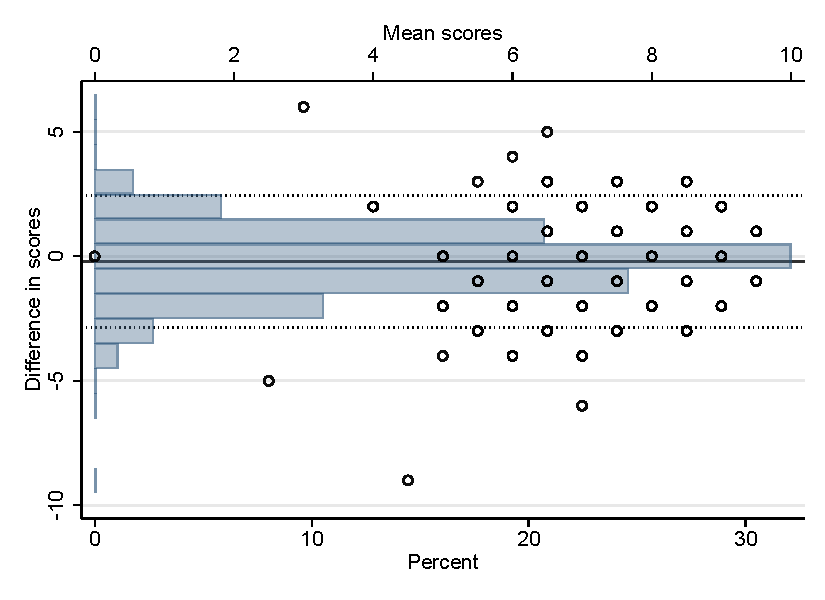
\includegraphics[width=\textwidth]{Figuras/bland_altman_total_12.pdf}
    \end{subfigure}
    \begin{subfigure}{0.5\textwidth}
        \caption{Total Score (1 vs 3)}
        \centering
        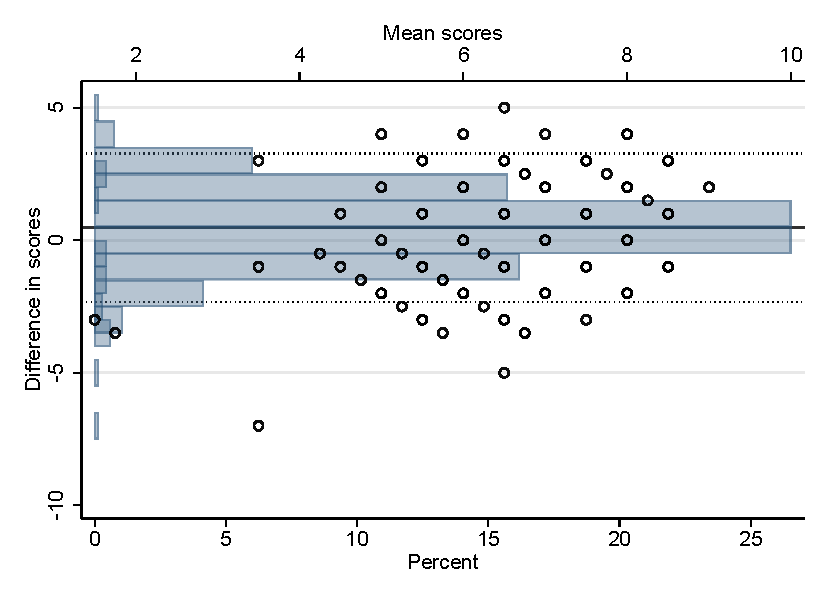
\includegraphics[width=\textwidth]{Figuras/bland_altman_total_13.pdf}
    \end{subfigure}
    \begin{subfigure}{0.5\textwidth}
        \caption{Total Score (2 vs 3)}
        \centering
        \includegraphics[width=\textwidth]{Figuras/bland_altman_total_23.pdf}
    \end{subfigure}
    
    \end{center}
    \scriptsize{ \noindent 
    \textit{Do file: }  \texttt{laywer\_scores\_p3\_f.do}}

\end{figure}


\subsection{ICC}

Bland and Altman make the point that any two methods that are designed to measure the same parameter (or property) should have good correlation when a set of samples are chosen such that the property to be determined varies considerably. A high correlation for any two methods designed to measure the same property could thus in itself just be a sign that one has chosen a widespread sample. A high correlation does not necessarily imply that there is good agreement between the two methods.


\begin{table}[H]
    \caption{ICC between raters}
    \label{icc_cor}
    \begin{center}
    \scriptsize{% Table generated by Excel2LaTeX from sheet 'total_cor'
\begin{tabular}{l|rrrrrrrrrrrrrl}
\toprule
\multicolumn{15}{c}{Individual ICC} \\
\midrule
      & 1     & 2     & 3     & 4     & 5     & 6     & 7     & 8     & 9     & 10    & 11    & 12    & 13    & \multicolumn{1}{r}{14} \\
\midrule
\midrule
Rater 1 & \multicolumn{1}{l}{} & \multicolumn{1}{l}{} & \multicolumn{1}{l}{} & \multicolumn{1}{l}{} & \multicolumn{1}{l}{} & \multicolumn{1}{l}{} & \multicolumn{1}{l}{} & \multicolumn{1}{l}{} & \multicolumn{1}{l}{} & \multicolumn{1}{l}{} & \multicolumn{1}{l}{} & \multicolumn{1}{l}{} & \multicolumn{1}{l}{} &  \\
Rater 2 & \cellcolor[rgb]{ .984,  .933,  .945}0.11 & \multicolumn{1}{l}{} & \multicolumn{1}{l}{} & \multicolumn{1}{l}{} & \multicolumn{1}{l}{} & \multicolumn{1}{l}{} & \multicolumn{1}{l}{} & \multicolumn{1}{l}{} & \multicolumn{1}{l}{} & \multicolumn{1}{l}{} & \multicolumn{1}{l}{} & \multicolumn{1}{l}{} & \multicolumn{1}{l}{} &  \\
Rater 3 & \cellcolor[rgb]{ .98,  .824,  .835}-0.01 & \cellcolor[rgb]{ .545,  .678,  .847}0.66 & \multicolumn{1}{l}{} & \multicolumn{1}{l}{} & \multicolumn{1}{l}{} & \multicolumn{1}{l}{} & \multicolumn{1}{l}{} & \multicolumn{1}{l}{} & \multicolumn{1}{l}{} & \multicolumn{1}{l}{} & \multicolumn{1}{l}{} & \multicolumn{1}{l}{} & \multicolumn{1}{l}{} &  \\
Rater 4 & \cellcolor[rgb]{ .976,  .643,  .655}-0.21 & \cellcolor[rgb]{ .91,  .933,  .973}0.26 & \multicolumn{1}{l}{} & \multicolumn{1}{l}{} & \multicolumn{1}{l}{} & \multicolumn{1}{l}{} & \multicolumn{1}{l}{} & \multicolumn{1}{l}{} & \multicolumn{1}{l}{} & \multicolumn{1}{l}{} & \multicolumn{1}{l}{} & \multicolumn{1}{l}{} & \multicolumn{1}{l}{} &  \\
Rater 5 & \cellcolor[rgb]{ .976,  .635,  .643}-0.22 & \cellcolor[rgb]{ .945,  .957,  .984}0.22 & \cellcolor[rgb]{ .565,  .69,  .851}0.64 & \cellcolor[rgb]{ .984,  .914,  .925}0.09 & \multicolumn{1}{l}{} & \multicolumn{1}{l}{} & \multicolumn{1}{l}{} & \multicolumn{1}{l}{} & \multicolumn{1}{l}{} & \multicolumn{1}{l}{} & \multicolumn{1}{l}{} & \multicolumn{1}{l}{} & \multicolumn{1}{l}{} &  \\
Rater 6 & \cellcolor[rgb]{ .663,  .761,  .886}0.53 & \cellcolor[rgb]{ .984,  .976,  .988}0.16 & \cellcolor[rgb]{ .984,  .914,  .925}0.09 & \cellcolor[rgb]{ .353,  .541,  .776}0.87 & \cellcolor[rgb]{ .973,  .976,  .996}0.19 & \multicolumn{1}{l}{} & \multicolumn{1}{l}{} & \multicolumn{1}{l}{} & \multicolumn{1}{l}{} & \multicolumn{1}{l}{} & \multicolumn{1}{l}{} & \multicolumn{1}{l}{} & \multicolumn{1}{l}{} &  \\
Rater 7 & \cellcolor[rgb]{ .953,  .965,  .988}0.21 & \cellcolor[rgb]{ .71,  .792,  .902}0.48 & \cellcolor[rgb]{ .882,  .914,  .965}0.29 & \cellcolor[rgb]{ .984,  .859,  .871}0.03 & \cellcolor[rgb]{ .98,  .831,  .843}0 & \cellcolor[rgb]{ .835,  .882,  .949}0.34 & \multicolumn{1}{l}{} & \multicolumn{1}{l}{} & \multicolumn{1}{l}{} & \multicolumn{1}{l}{} & \multicolumn{1}{l}{} & \multicolumn{1}{l}{} & \multicolumn{1}{l}{} &  \\
Rater 8 & \cellcolor[rgb]{ .98,  .831,  .843}0 & \cellcolor[rgb]{ .745,  .82,  .918}0.44 & \cellcolor[rgb]{ .863,  .902,  .957}0.31 & \cellcolor[rgb]{ .671,  .765,  .89}0.52 & \cellcolor[rgb]{ .49,  .639,  .827}0.72 & \cellcolor[rgb]{ .984,  .898,  .906}0.07 & \cellcolor[rgb]{ .592,  .71,  .863}0.61 & \multicolumn{1}{l}{} & \multicolumn{1}{l}{} & \multicolumn{1}{l}{} & \multicolumn{1}{l}{} & \multicolumn{1}{l}{} & \multicolumn{1}{l}{} &  \\
Rater 9 & \cellcolor[rgb]{ .843,  .886,  .949}0.33 & \cellcolor[rgb]{ .627,  .733,  .875}0.57 & \cellcolor[rgb]{ .565,  .69,  .851}0.64 & \cellcolor[rgb]{ .855,  .894,  .953}0.32 & \cellcolor[rgb]{ .647,  .749,  .882}0.55 & \cellcolor[rgb]{ .855,  .894,  .953}0.32 & \cellcolor[rgb]{ .98,  .761,  .773}-0.08 & \cellcolor[rgb]{ .71,  .792,  .902}0.48 & \multicolumn{1}{l}{} & \multicolumn{1}{l}{} & \multicolumn{1}{l}{} & \multicolumn{1}{l}{} & \multicolumn{1}{l}{} &  \\
Rater 10 & \cellcolor[rgb]{ .737,  .812,  .914}0.45 & \cellcolor[rgb]{ .8,  .855,  .933}0.38 & \cellcolor[rgb]{ .984,  .886,  .898}0.06 & \cellcolor[rgb]{ .984,  .851,  .863}0.02 & \cellcolor[rgb]{ .98,  .788,  .8}-0.05 & \cellcolor[rgb]{ .98,  .831,  .843}0 & \cellcolor[rgb]{ .984,  .871,  .878}0.04 & \cellcolor[rgb]{ .984,  .859,  .871}0.03 & \cellcolor[rgb]{ .98,  .725,  .733}-0.12 & \multicolumn{1}{l}{} & \multicolumn{1}{l}{} & \multicolumn{1}{l}{} & \multicolumn{1}{l}{} &  \\
Rater 11 & \multicolumn{1}{l}{} & \multicolumn{1}{l}{} & \multicolumn{1}{l}{} & \cellcolor[rgb]{ .984,  .922,  .933}0.1 & \cellcolor[rgb]{ .937,  .953,  .984}0.23 & \multicolumn{1}{l}{} & \cellcolor[rgb]{ .984,  .859,  .871}0.03 & \multicolumn{1}{l}{} & \cellcolor[rgb]{ .984,  .933,  .945}0.11 & \multicolumn{1}{l}{} & \multicolumn{1}{l}{} & \multicolumn{1}{l}{} & \multicolumn{1}{l}{} &  \\
Rater 12 & \cellcolor[rgb]{ .725,  .804,  .91}0.46 & \cellcolor[rgb]{ .984,  .914,  .925}0.09 & \cellcolor[rgb]{ .91,  .933,  .973}0.26 & \cellcolor[rgb]{ .937,  .953,  .984}0.23 & \cellcolor[rgb]{ .792,  .851,  .933}0.39 & \cellcolor[rgb]{ .98,  .816,  .827}-0.02 & \cellcolor[rgb]{ .882,  .914,  .965}0.29 & \cellcolor[rgb]{ .6,  .714,  .863}0.6 & \cellcolor[rgb]{ .98,  .698,  .71}-0.15 & \cellcolor[rgb]{ .98,  .808,  .816}-0.03 & \multicolumn{1}{l}{} & \multicolumn{1}{l}{} & \multicolumn{1}{l}{} &  \\
Rater 13 & \cellcolor[rgb]{ .882,  .914,  .965}0.29 & \cellcolor[rgb]{ .984,  .976,  .988}0.16 & \cellcolor[rgb]{ .855,  .894,  .953}0.32 & \cellcolor[rgb]{ .984,  .859,  .871}0.03 & \cellcolor[rgb]{ .973,  .412,  .42}-0.47 & \cellcolor[rgb]{ .98,  .753,  .761}-0.09 & \cellcolor[rgb]{ .98,  .808,  .816}-0.03 & \cellcolor[rgb]{ .984,  .859,  .871}0.03 & \cellcolor[rgb]{ .98,  .733,  .745}-0.11 & \cellcolor[rgb]{ .984,  .851,  .863}0.02 & \multicolumn{1}{l}{} & \cellcolor[rgb]{ .984,  .843,  .855}0.01 & \multicolumn{1}{l}{} &  \\
Rater 14 & \cellcolor[rgb]{ .984,  .886,  .898}0.06 & \cellcolor[rgb]{ .945,  .957,  .984}0.22 & \cellcolor[rgb]{ .835,  .882,  .949}0.34 & \cellcolor[rgb]{ .827,  .875,  .945}0.35 & \cellcolor[rgb]{ .863,  .902,  .957}0.31 & \cellcolor[rgb]{ .973,  .976,  .996}0.19 & \cellcolor[rgb]{ .98,  .984,  1}0.18 & \cellcolor[rgb]{ .984,  .941,  .953}0.12 & \cellcolor[rgb]{ .855,  .894,  .953}0.32 & \cellcolor[rgb]{ .984,  .922,  .933}0.1 & \cellcolor[rgb]{ .973,  .51,  .518}-0.36 & \cellcolor[rgb]{ .984,  .961,  .973}0.14 & \cellcolor[rgb]{ .984,  .843,  .855}0.01 &  \\
\bottomrule
\bottomrule
\end{tabular}%
}
    \end{center}
  \scriptsize{ \noindent 
    \textit{Do file: }  \texttt{laywer\_scores\_p3\_f.do}}
\end{table}




\section{Determinants of measures of quality}

We tried to predict the ratings (continuous variable 1-10)  with casefile variables, but we fail to do so even with non-linear ML models. If instead we tried to predict a binary variable "above median", results are similar - we achieve an accuracy of 0.58). This suggest there is something on the initial lawsuit that is not captured by the coded variables. For instance, something about the wording, how a lawyer asks for benefits, etc. The next table shows out-of-sample statistics. In-sample we get a R-squared of 0.2 for the Boosting models.



\begin{figure}[H]%-------------------------------------------
 \centering
 \caption{OOS measures of fit using initial casefile variables}
 \includegraphics[width=\textwidth]{Figuras/oos_X_HD.png}
 \label{fig:3}
\end{figure}

\begin{figure}[H]%-------------------------------------------
 \centering
 \caption{OOS measures of fit using hearing variables}
 \includegraphics[width=\textwidth]{Figuras/oos_Z_HD.png}
 \label{fig:3}
\end{figure}


\begin{figure}[H]%-------------------------------------------
 \centering
 \caption{OOS measures of fit using all variables}
 \includegraphics[width=\textwidth]{Figuras/oos_W_HD.png}
 \label{fig:3}
\end{figure}





For the subjective measure of quality, this are the results

\begin{figure}[H]%-------------------------------------------
 \centering
 \caption{OOS measures of fit using initial casefile variables}
 \includegraphics[width=\textwidth]{Figuras/oos_X_p3.png}
 \label{fig:3}
\end{figure}

\begin{figure}[H]%-------------------------------------------
 \centering
 \caption{OOS measures of fit using hearing variables}
 \includegraphics[width=\textwidth]{Figuras/oos_Z_p3.png}
 \label{fig:3}
\end{figure}


\begin{figure}[H]%-------------------------------------------
 \centering
 \caption{OOS measures of fit using all variables}
 \includegraphics[width=\textwidth]{Figuras/oos_W_p3.png}
 \label{fig:3}
\end{figure}

Here are the most "important" variables in terms of predictive power according to the Gradient Boosting

\begin{figure}[H]%-------------------------------------------
 \centering
 \caption{Variable importance}
 \includegraphics[width=0.5\textwidth]{Figuras/importance.png}
 \label{fig:3}
\end{figure}

\section{Latent model}

\section{Objective measures vs Subjective measures}


There is difficulty in contrasting both measures of quality, since in principle we are dealing with distinct datasets. To overcome this, we aim to xxxx...

\begin{figure}[H]%-------------------------------------------
 \centering
 \caption{Objective vs subjective}
 \includegraphics[width=\textwidth]{Figuras/obj_vs_sub.png}
 \label{fig:3}
\end{figure}





%\singlespacing
%\setlength\bibsep{0pt}
\bibliographystyle{aea}
\bibliography{bibliography.bib}



\clearpage

\onehalfspacing


%-------------------------------------------------------------




\clearpage


% \begin{figure}[hp]%-----------------------------------------
%  \centering
%  \captionof{table}{Summary Statistics and Balance}
%  \includegraphics[width=.8\textwidth]{Table2.png}
%  \caption*{Notes: The table shows goodness-of-fit statistics: correlation of predicted vs. actual subjective quality; mean square error and out-of-sample R square in a regression of predicted vs. actual subjective quality.}
%  \label{tab:2}
% \end{figure}%-----------------------------------------------


%\begin{figure}[hp]
%  \centering
%  \includegraphics[width=.8\textwidth]{../fig/placeholder.pdf}
%  \caption{Placeholder}
%  \label{fig:placeholder}
%\end{figure}




\clearpage



\end{document}